\section{Estudi d'ablació: resultats}\label{sec:resultats}

\begin{figure}[htbp]
  \centering
  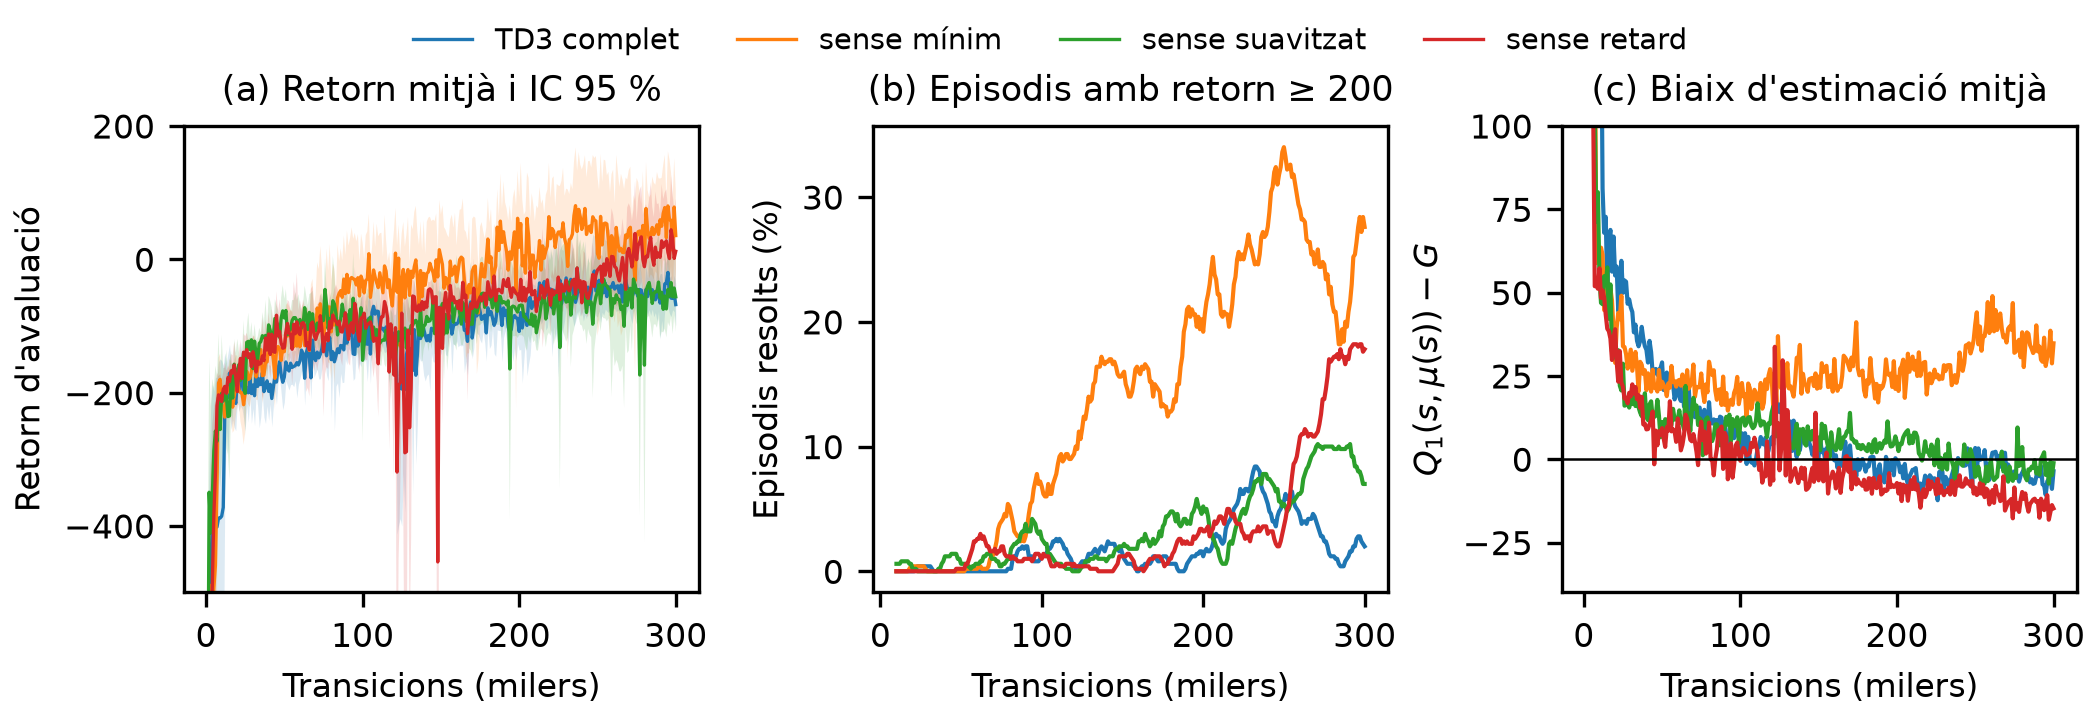
\includegraphics[width=\linewidth]{img/fig_ablacio.png}
  \caption{Ablació de TD3, 10 llavors per variant. (a) Retorn d'avaluació mitjà entre llavors cada 1.000 transicions, amb IC del 95~\% per \emph{bootstrap}; l'eix vertical està retallat a −500. (b) Percentatge d'episodis d'avaluació amb retorn ≥ 200 (mitjana mòbil de 10 avaluacions). (c) Biaix mitjà $Q_1(s,\mu(s))-G$.}
  \label{fig:ablacio}
\end{figure}

\begin{table}[htbp]
  \centering
  \small
  \caption{Ablació, 10 llavors per variant (mitjana ± desviació estàndard). Δ L10: diferència aparellada respecte de TD3 complet; $p$ Holm: test de permutació aparellat exacte amb correcció de Holm. Sobre les últimes 10 avaluacions: Resolts, episodis amb retorn ≥ 200; Truncades, avaluacions amb els cinc episodis truncats a 1.000 passos; Biaix, $Q_1(s,\mu(s))-G$.}
  \label{tbl:ablacio}
  \setlength{\tabcolsep}{2.5pt}
  \begin{tabular}{lrrrrrrr}
    \toprule
    Variant & L10 & AUC/T & Δ L10 [IC 95~\%] & $p$ Holm & Resolts & Truncades & Biaix \\
    \midrule
    TD3 complet & −51,3 ± 45,9 & −115,2 ± 43,5 & --- & --- & 2,0~\% & 65~\% & −6,4 ± 7,5 \\
    Sense mínim & 55,4 ± 110,1 & −45,8 ± 67,0 & +106,6 [27,5, 177,6] & 0,088 & 27,6~\% & 25~\% & +32,2 ± 18,2 \\
    Sense suavitzat & −54,6 ± 95,1 & −95,6 ± 48,4 & −3,4 [−51,1, 55,1] & 0,902 & 7,0~\% & 70~\% & −2,2 ± 13,3 \\
    Sense retard & 19,7 ± 110,5 & −86,8 ± 45,3 & +70,9 [11,2, 142,7] & 0,152 & 17,8~\% & 57~\% & −14,4 ± 11,5 \\
    \bottomrule
  \end{tabular}
\end{table}

Cap variant arriba al llindar de 200 en mitjana, i les corbes de retorn de sense mínim i sense retard encara pugen als 300.000 passos, mentre que la de TD3 complet és gairebé plana des dels 250.000 (Figura~\ref{fig:ablacio}a). La variant sense mínim obté la L10 i l'AUC/T més altes (Taula~\ref{tbl:ablacio}) i supera TD3 complet en 8 de les 10 llavors, amb $p = 0{,}029$ sense corregir i $p = 0{,}088$ amb Holm. La variant sense retard també millora la mitjana en 8 de 10 llavors ($p = 0{,}152$ amb Holm), però la seva mediana (−27,7) queda molt per sota de la mitjana (19,7) perquè dues llavors, amb una L10 de 239,8 i 184,7, concentren la millora. Sense suavitzat, en canvi, no es distingeix de TD3 complet, i amb la correcció de Holm cap diferència és significativa al 5~\%.

La fracció d'episodis resolts separa més les variants (Figura~\ref{fig:ablacio}b). Cap llavor de TD3 complet arriba a resoldre el 50~\% dels episodis, i quatre de sense mínim hi arriben o el superen. La diferència es manté en les cinc condicions inicials d'avaluació: sense mínim en resol entre el 21~\% i el 33~\% de cada condició, i TD3 complet entre el 0~\% i el 5~\%. A canvi, sense mínim és la variant més inestable, amb 73 caigudes de més de 200 punts entre avaluacions consecutives després dels 50.000 passos, per 17 de TD3 complet.

El biaix final (Figura~\ref{fig:ablacio}c) és proper a zero o negatiu a les tres variants que conserven el mínim. L'única que sobreestima és sense mínim, amb un valor proper al de DDPG (secció~\ref{sec:ddpg}). Dins de cada variant, les llavors amb més biaix tendeixen a acabar amb menys retorn: la correlació de Spearman entre el biaix i la L10 va de −0,24 a −0,72 segons la variant (10 llavors cadascuna).
